\chapter{ Analysis And Design} 

In this chapter, we outline the project planning process for the development of an AI-powered mental health application. We delineate the functional and non-functional requirements identified through extensive research, and detail the strategies employed to address these requirements.

\section{Functional Requirements}
Functional requirements delineate the specific features and capabilities that our application must possess to meet the needs and expectations of its users.
\subsection{Login and Register}

The application provides a user-friendly interface for new users to register and existing users to sign in.

\paragraph{User Registration}

If a user wants to register, they can do so in one of the following ways:

\begin{itemize}
    \item \textbf{Creating a New Account:} Users can create a new account by providing necessary details such as username, password, email, and other required information. 
    \item \textbf{Signing Up Using Google or Facebook:} Users have the option to sign up using their existing Google or Facebook accounts. This option simplifies the registration process by allowing users to authenticate using their social media credentials.
\end{itemize}

\paragraph{User Login}

Users who already have an account can sign in to the application by:

\begin{itemize}
    \item \textbf{Standard Login:} Entering their registered username and password.
    \item \textbf{Social Media Login:} Logging in through their Google or Facebook accounts, provided they have previously registered using these credentials.
\end{itemize}

\begin{figure}[h]
    \includegraphics[width=\columnwidth]{login}
    \caption{Login and Registration Flow Digram}  
    \centering
    \end{figure}



\subsection{Chat with AI}

The application allows users to initiate and engage in chat sessions with the AI, enabling them to have meaningful conversations and seek mental health support.

\paragraph{Users can :}

\begin{itemize}
    \item \textbf{Starting a New Conversation:} Users can click on the "Start Chat" button to initiate a new conversation with the AI. 
\end{itemize}

\subsection{Persona List}

The Persona List feature allows users to create and manage a list of characters with whom they can engage in conversations. The application saves all interactions with each character, providing a personalized experience.

\paragraph{Users can:}

\begin{itemize}
    \item \textbf{Create New Persona:} Add new personas by providing Persona details such as name.
    \item \textbf{Edit Existing Persona:} Modify details of existing personas to update their characteristics.
    \item \textbf{Delete Persona:} Remove Personas from the list if they are no longer needed.
\end{itemize}



    \subsection{Chat List}

Within each persona, the Chat List feature provides a detailed list of conversations the user has had with that character. This organization helps users manage and review their interactions effectively.

\paragraph{Users can:}

\begin{itemize}
    \item \textbf{Select a Persona:} Choose a persona from the Persona List to view all associated conversations.
    ry in the Chat List includes the date and time of the conversation, providing a chronological overview.
    \item \textbf{Access Detailed Chats:} Click on an entry to view the full conversation, allowing users to revisit and analyze past interactions.
\end{itemize}

\subsection{Previous Conversations}

The application provides a feature for users to view their previous interactions, allowing them to track and reference past conversations with ease.

\paragraph{Users can:}

\begin{itemize}
    \item \textbf{View Details:} Each conversation entry includes the name of the interaction, duration, and date. This provides users with a quick overview of their past chats.
    \item \textbf{Select and Review:} Users can select a conversation to review the chat history, facilitating continuity and reference to past discussions.
\end{itemize}

\subsection{Positive Card}

The application includes an interactive \textit{Positive Card} feature designed to enhance the user's mood and foster positivity.

\paragraph{Functionality of the Positive Card}

The Positive Card provides:

\begin{itemize}
    \item \textbf{Interactive Content:} Engaging content such as motivational quotes, positive affirmations, or uplifting messages tailored to improve the user's mood.

\end{itemize}

\subsection{Mood Tracker}

The Mood Tracker feature allows users to monitor their emotional state over time, helping them identify their emotions in the period of using the app and effectively manage their mental health.

\paragraph{Users can:}

\begin{itemize}
 \item \textbf{Log emotional states:} Record your mood at different times throughout the day or week, or choose from predefined categories.
 \item \textbf{View Mood History:} Access a historical record of your recorded moods, presented in an intuitive interface that includes graphs or charts showing mood trends over time.

\end{itemize}


\section{Non-Functional Requirements}
Non-functional requirements encompass the attributes that characterize the overall performance, usability, and scalability of our application.

\subsection{Security and Privacy}

Ensuring the security and privacy of user data is paramount in our application. We implement robust security measures to maintain the confidentiality of users and ensure complete privacy. Data protection is enforced through secure communication channels and encryption between the server, the user, and the AI model.

\paragraph{Data Protection}

\begin{itemize}
    \item \textbf{Encryption:} All user data is encrypted during transmission and storage to prevent unauthorized access.
    \item \textbf{Secure Authentication:} Implement secure authentication mechanisms such as multi-factor authentication to verify user identity.
    \item \textbf{Compliance:} Adhere to privacy regulations and standards to ensure user data is handled responsibly and legally.
\end{itemize}

\subsection{Speak Comfortably}

Our application supports the Arabic language, enabling users to communicate comfortably and express themselves accurately in their native language. This language support is crucial for effective interaction and user satisfaction.

\subsection{Speed Of Response}

our application is designed to provide rapid responses to user inputs, facilitating a smooth and continuous conversation experience without long wait times.

\subsection{Usability and User Experience}

Our application features a user-friendly interface that is simple and easy to navigate, allowing users to interact with the application effortlessly.

\paragraph{User-Centric Design}

\begin{itemize}
    \item \textbf{Intuitive Interface:} We  Designed an interface that is easy to learn and use, with clear navigation and well-organized elements.
    \item \textbf{Aesthetic Appeal:}we  Ensured the visual design is appealing and enhances the user experience.
 
\end{itemize}



\section{Implementation Strategies}

To address the identified functional and non-functional requirements, various implementation strategies and technologies are employed in the development of the application.

\subsection{Cross-Platform Development with Flutter}

Utilizing Flutter for cross-platform development enables applications to reach a broader audience across different devices and operating systems, enhancing accessibility and user engagement. Flutter’s unique approach to building natively compiled applications for mobile, web, and desktop from a single codebase ensures that the application can cater to a diverse user base without needing separate versions for each platform. This strategy saves significant time and resources \cite{flutter_overview}.

\subsection{Advantages of Flutter} 

\paragraph{Broader Accessibility} Flutter allows the application to be compatible with various operating systems, including iOS, Android, Windows, macOS, Linux, and Web. This wide range of support ensures that users can access the application regardless of their preferred device or platform .

\paragraph{Consistent User Experience} Flutter provides a rich set of customizable widgets and its own rendering engine, enabling the creation of a consistent user experience across different devices. This consistency is crucial for delivering a seamless and unified user interface and interaction flow, which enhances user satisfaction and engagement. The ability to achieve pixel-perfect UI on various platforms ensures that users enjoy a similar experience, irrespective of the device they use \cite{flutter_cons_pros}.

\paragraph{Cost-Efficiency} Flutter’s approach to a single codebase for multiple platforms significantly reduces development costs compared to creating and maintaining separate codebases for each platform. This cost-efficiency extends to updates and maintenance since changes can be implemented once and reflected across all platforms, eliminating the need for redundant development efforts \cite{codecademy_flutter}.

\paragraph{Faster Time-to-Market} Flutter accelerates the deployment process by allowing the development of a single codebase that can be compiled into applications for multiple platforms. This rapid development and deployment capability are crucial for addressing user needs promptly and maintaining competitiveness in the market. Flutter's hot-reload feature further speeds up the development process by enabling real-time changes without restarting the app \cite{flutter_hot_reload}.

\paragraph{Simplified Testing} With a unified codebase in Flutter, the testing process is streamlined, allowing developers to identify and address issues more efficiently. This simplification ensures higher quality and reliability of the application across all supported platforms. Additionally, Flutter’s comprehensive testing framework supports unit, widget, and integration testing, facilitating thorough testing processes \cite{flutter_testing}.



\subsection{programming languages}

The choice of programming languages plays a crucial role in the development of the application. Go is utilized for server-side programming due to its efficiency, concurrency support, and scalability, while Python is leveraged for artificial intelligence programming owing to its extensive libraries and frameworks tailored for machine learning and natural language processing tasks.

\subsection{Server-Side Programming with Go}

\paragraph{Efficiency and Performance:} Go (Golang) offers excellent performance due to its compiled nature and efficient garbage collection. This performance is crucial for handling large volumes of requests and ensuring smooth operation of the application \cite{golang_efficiency}.

\paragraph{Concurrency Support:} Go’s native support for concurrency through goroutines allows the application to manage multiple processes simultaneously, enhancing the system’s ability to handle concurrent user interactions and background tasks \cite{golang_concurrency}.

\paragraph{Scalability:} Go’s design principles and simplicity make it well-suited for building scalable server-side applications, ensuring the AI mental health application can grow and adapt to increasing user demands \cite{golang_scalability}.

\subsection{AI and Machine Learning with Python}

\paragraph{Extensive Libraries:} Python is chosen for artificial intelligence programming due to its rich ecosystem of libraries and frameworks, such as TensorFlow, Keras, and scikit-learn. These tools provide robust support for developing and deploying AI models, including those for natural language processing and sentiment analysis \cite{tensorflow, keras, scikit_learn}.

\paragraph{Ease of Integration:} Python’s flexibility and ease of integration with other technologies facilitate the incorporation of AI capabilities into the application, enabling the development of sophisticated mental health support features \cite{python_integration}.


\section{System analysis through formal diagrams }

The next section provides a detailed analysis of the system through Four formal diagrams and a wireframe. These diagrams will delve into different aspects of the system, including an outline of what the application looks like, users interacting with it (Use Cases), its internal processes (activities), and the flow of communications between components (sequences). In addition, they will identify the basic elements (Class Digram) of the system and its different operational states.

\subsection{Wireframe}
In this wireframe, we present the initial design of the application and present the most important requirements that make up the application

\begin{figure}[h]
\includegraphics[width=0.5\textwidth, height=0.5\textheight]{wf}
\caption{Wireframe for the main screen of application}
\centering
\end{figure}

\subsection{Use Case Diagram }
The use case diagram depicts an app "WANAS," with the user as the central actor. It outlines the actions users can perform within the system, such as registering, logging in, editing their profiles, starting a chat, interacting with personas, tracking their mood, accessing tips, deleting their account, and logging out. There are also extended use cases, including editing passwords, email, and pictures, suggesting a focus on user management and personalization.

\begin{figure}[h]
    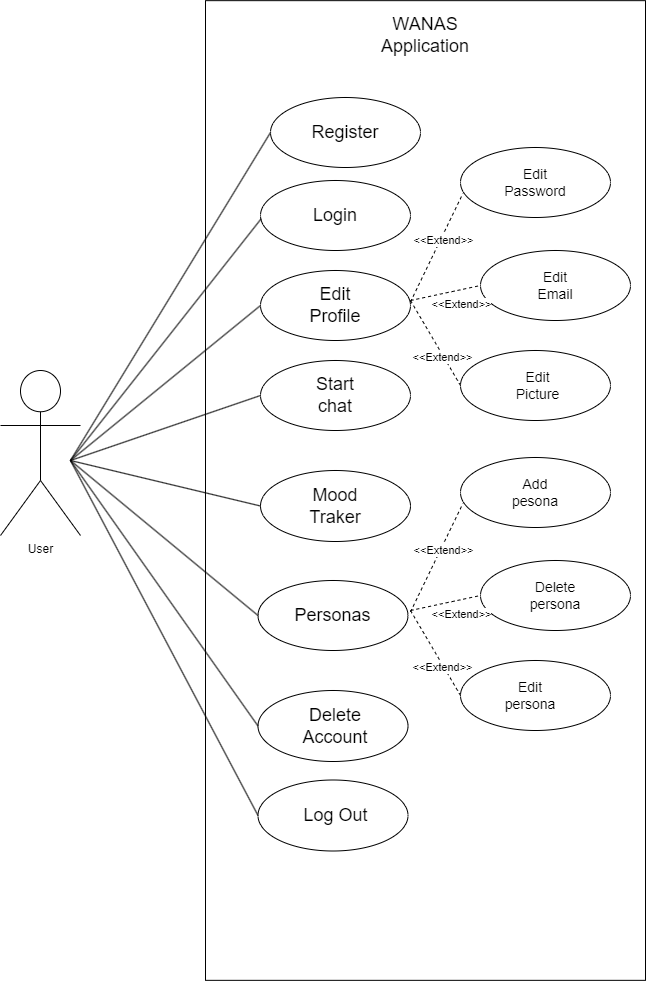
\includegraphics[width=0.8\textwidth, height=0.7\textheight]{fuc}
    \caption{Use Case for application}
    \centering
    \end{figure}

 
    \subsection{Activity Diagram }
    The flow of actions that the user can perform is depicted in the following figure: 
    \begin{itemize}
        \item  It displays the flow of the Login and Register processes. The user can select to reach the home page by registering to create a new account or by logging in if he already has one. Without validating, the user won't be able to view the home page.
        \item  After logging in user can make changes in his profile , start chat , personas list , choose mood.
     
    \end{itemize}
    
    \begin{figure}[h]
        \includegraphics[width=0.8\textwidth, height=0.7\textheight]{acdi}
        \caption{Activity diagram for application}
        \centering
        \end{figure}
    


      \subsection{Sequence Diagram }
      The sequence diagram shows the interactions between a user and a system in a chat application. The user starts by logging in or registering. After successful authentication, the user can create a chat, choose a state, edit the state, edit their profile picture, edit their email, or edit their password. The system interacts with the database to save and retrieve user data and chat information. The mood tracker and the profile features are also represented in the diagram.
    
    
            \begin{figure}[h]
                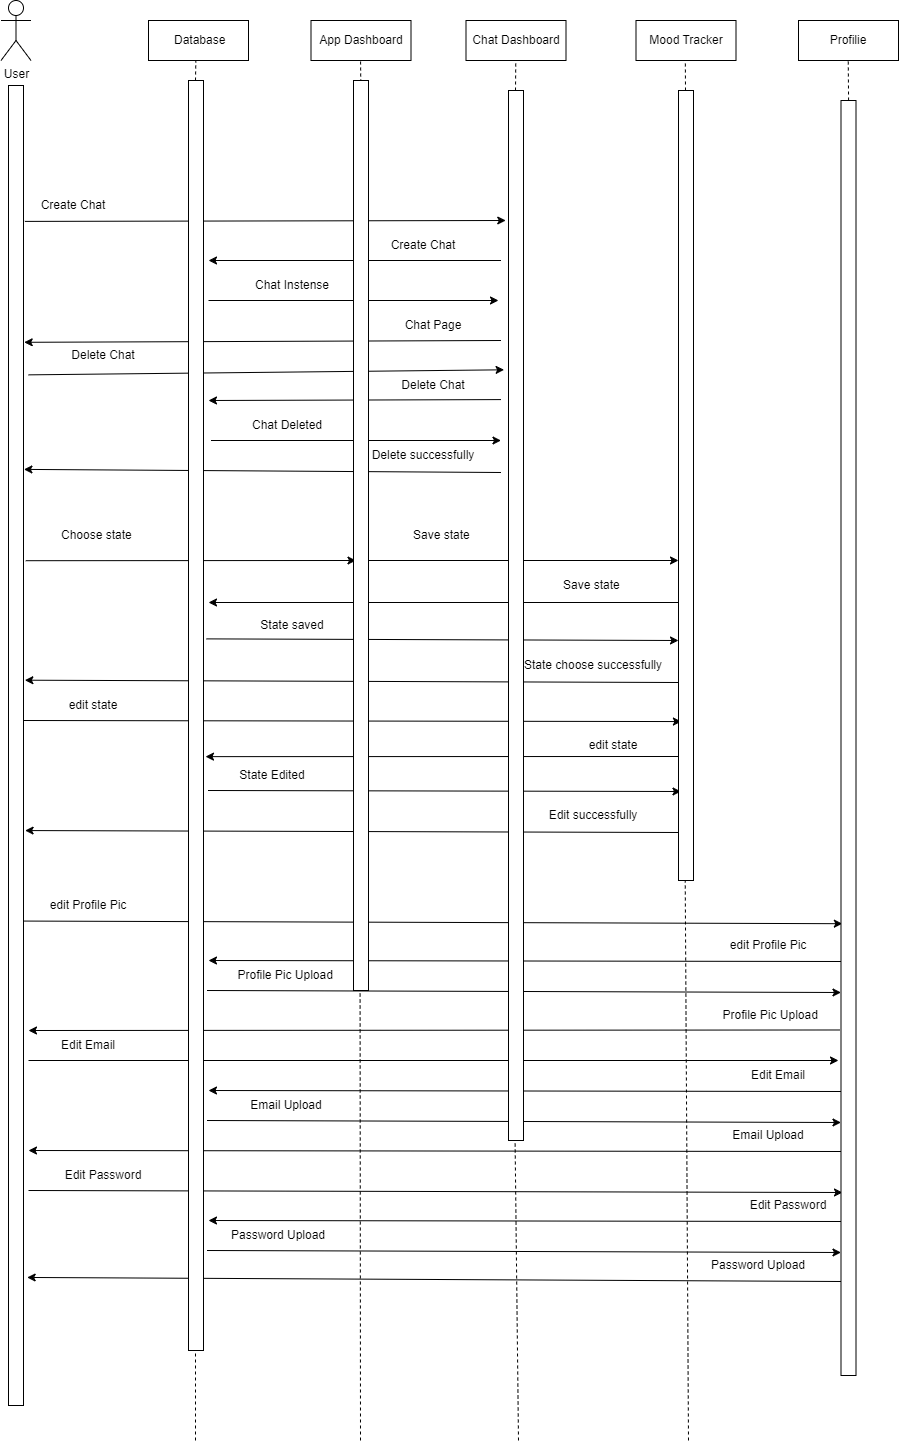
\includegraphics[width=0.8\textwidth, height=0.7\textheight]{seq}
                \caption{Sequence diagram for application}
                \centering
                \end{figure}
 \subsection{Class Diagram }
 The following figures represents the functions and attributes of the four main classes that the system use :
 \begin{itemize}
 \item  Persona .
 \item  User.
 \item  Message .
 \item  Chatbot.
\end{itemize}
  \begin{figure}[h]
       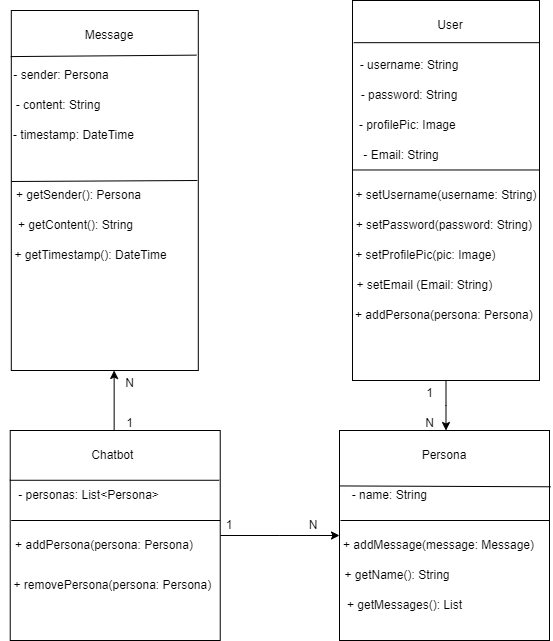
\includegraphics[width=0.7\textwidth, height=0.5\textheight]{ccd}
     \caption{Class diagram for application}
     \centering
    \end{figure}
          
